\section{Display}
	\begin{figure}[h]
		\centering 
		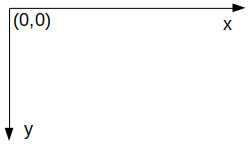
\includegraphics[width=5cm]{images/EV3-CoordSystem.png}
		\caption{Koordinatensystems des Displays}
	\end{figure}
	\begin{table}[h]
		\begin{tabular}{|p{0.2\textwidth}| p{0.7\textwidth}|}
			\hline
			Display& lejos.hardware.lcd.LCD
			\\ \hline 
		\end{tabular}
		\caption{ben"otigter Import}
	\end{table}
	
	\begin{table}[H]
		\begin{tabular}{|p{0.2\textwidth}| p{0.7\textwidth}|}
			\hline
			drawString(String str, int x, int y)& Zeigt einen Text an, beginnend in Spalte x und Zeile y \\ \hline 
			drawInt(int i, int x, int y) &  Zeigt eine Ganzzahl an, beginnend in Spalte x und Zeile y\\ \hline 
			clear() & l"oscht den Inhalt des Displays\\ \hline
			clear(int y)& l"oscht den Inhalt der y-ten Zeile \\ \hline 
			scroll()& verschiebt den Inhalt um eine Zeile nach oben \\ \hline 
		\end{tabular}
		\caption{wichtige Methoden}
	\end{table}

	Das Koordinatensystem auf dem Display hat seinen Ursprung (0,0) oben links und geht in x-Richtung nach rechts 16 Spalten und in y-Richtung nach unten 8 Zeilen. \\ \\
	Das Display wird angesprochen mit: \textbf{LCD.Methode}\\
	\textbf{Bsp.: LCD.drawString(\glqq Hallo Welt!\grqq{}, 0, 0);}
